\documentclass{article}
\usepackage[utf8]{inputenc}
\usepackage{multicol}
\usepackage[none]{hyphenat}
\usepackage{amsmath}
\usepackage{amssymb}
\usepackage{listings}
\usepackage{hyperref}

\usepackage{glossaries}
\makeglossaries

\usepackage{xcolor}

\usepackage[verbose=true,letterpaper]{geometry}
\AtBeginDocument{
  \newgeometry{
    textheight=9in,
    textwidth=6.5in,
    top=1in,
    headheight=14pt,
    headsep=25pt,
    footskip=30pt
  }
}

\definecolor{codegreen}{rgb}{0,0.6,0}
\definecolor{codegray}{rgb}{0.5,0.5,0.5}
\definecolor{codepurple}{rgb}{0.58,0,0.82}
\definecolor{backcolour}{rgb}{0.95,0.95,0.92}

\lstdefinestyle{mystyle}{
    backgroundcolor=\color{backcolour},   
    commentstyle=\color{codegreen},
    keywordstyle=\color{magenta},
    numberstyle=\tiny\color{codegray},
    stringstyle=\color{codepurple},
    basicstyle=\ttfamily\footnotesize,
    breakatwhitespace=false,         
    breaklines=true,                 
    captionpos=b,                    
    keepspaces=true,                 
    numbers=left,                    
    numbersep=5pt,                  
    showspaces=false,                
    showstringspaces=false,
    showtabs=false,                  
    tabsize=2
}

\lstset{style=mystyle}

\usepackage{graphicx}
\graphicspath{ {./images/} }

\title{A REPORT \\ ON \\ \textbf{DEEP REINFORCEMENT LEARNING IN \\ SUPPLY CHAIN MANAGEMENT} \\ \large{BY}}

\author{{Aditya Chopra} \and {2019A7PS0178H}}


\begin{document}

\begin{titlepage}
    \begin{center}
        \vspace*{1cm}

        \large\textbf{A Report \\ On}

        \vspace{0.5cm}

        \LARGE\textbf{DEEP REINFORCEMENT LEARNING IN \\ SUPPLY CHAIN MANAGEMENT}

        \vspace{0.5cm}

        \large By

        \vspace{1.5cm}

        \textbf{Aditya Chopra \hfill 2019A7PS0178H}

        \vspace{1.5cm}

        \large At

        \vspace{0.5cm}
        \textbf{Happiest Minds Technologies}

        \vspace{0.5cm}
        A Practice School - I Station of

        \vspace{0.8cm}
        \includegraphics{bits_logo.png}
        \vspace{0.8cm}

        \Large
        \textbf{BIRLA INSTITUTE OF TECHNOLOGY AND SCIENCE, PILANI}

        \textbf{(July, 2021)}

    \end{center}

\end{titlepage}

\begin{titlepage}
    \begin{center}
        \vspace*{1cm}

        \large\textbf{A Report \\ On}

        \vspace{0.5cm}

        \LARGE\textbf{DEEP REINFORCEMENT LEARNING IN \\ SUPPLY CHAIN MANAGEMENT}

        \vspace{0.5cm}

        \large By

        \vspace{1.5cm}

        \textbf{Aditya Chopra \hfill 2019A7PS0178H \hfill Computer Science Eng.}

        \vspace{0.5cm}
        \Large\textbf{Prepared In Partial Fulfillment of the \\ Practive School - I \\ Course No. BITS F221}

        \vspace{1cm}

        \large At

        \vspace{0.5cm}
        \textbf{Happiest Minds Technologies}

        \vspace{0.5cm}
        A Practice School - I Station of

        \vspace{0.8cm}
        \includegraphics{bits_logo.png}
        \vspace{0.8cm}

        \Large
        \textbf{BIRLA INSTITUTE OF TECHNOLOGY AND SCIENCE, PILANI}

        \textbf{(July, 2021)}

    \end{center}

\end{titlepage}

\vspace*{\fill}
\section*{\begin{center}Acknowledgements\end{center}}

I would like to express my sincerest gratitude to my PS instructor Dr. Ramakrishna Dantu for giving us his valuable time to provide me the required guidance wherever required. I would also like to thank my technical supervisor and metor, Mr. Samrat Sengupta as his input proved to be very vital for the project and Project Manager, Mr Andrew Anand for their valuable feedback. I would like to thank BITS PS Division and Administration for providing me with such a wonderful opportunity to apply my course knowledge on real life applications and get hands on experience. I am indebted for all the help and guidance that I have received.
\vspace*{\fill}

\pagebreak


\section*{\begin{center}BIRLA INSTITUTE OF TECHNOLOGY AND SCIENCE \\ PILANI, RAJASTHAN\end{center}}

\vspace{1.5cm}

\textbf{Station}: Happiest Minds Technologies \hspace*{3cm} \textbf{Centre}: Bangalore \\
\textbf{Duration}: 7 Weeks (46 Days) \hspace*{4.25cm} \textbf{Date of Start}: June 8, 2021 \\
\textbf{Date of Report Submission}: July 23, 2021

\vspace{1cm}
\textbf{Title of the Project: Deep Reinforcement Learning in Supply Chain Management}

\vspace{1cm}
\textbf{Aditya Chopra \hfill 2019A7PS0178H \hfill Computer Science Eng.}

\vspace{1cm}
\textbf{Name and Designation of Expert:}
\begin{enumerate}
    \item Samrat Sengupta, Senior Lead Data Scientist
    \item Andrew Anand, Director (CoE Analytics)
\end{enumerate}
\vspace{1cm}
\textbf{Name of the PS Faculty}: Dr. Ramakrishna Dantu \\
\textbf{Keywords}: \emph{CoE Analytics, Deep Reinforcement Learning, SQ Policy, Supply Chain Management} \\
\textbf{Project Area}: Deep Reinforcement Learning, Supply Chain Management \\ \\
\textbf{Abstract}: \\
In the past few years, Deep Learning has made ceratin strides with new models and architectures creating State of the Art on a daily basis. Deep Reinforcement Learning has consequently made incredible progress over the past decade, with the introduction of continuous control models that can surpass human performance. Supply Chain Management is such a case of a continuous control problem. A supply Chain must optimize the resource allocation, distribution and storage of raw materials, intermediaries and final products to minimize delays and maximise profits, or returns. This optimization problem where decisions must be taken dynamically is perfectly suited for Reinforcement Learning. We look at the use of continuous control models such as Deep Deterministic Policy Gradients \cite{lillicrap_continuous_2019}, Twin Delayed Deep Determininstic Policy Gradients\cite{fujimoto_addressing_2018}, and try to improve the returns gained over an episode. These results are compared to the Baselines determined using traditional methods of Supply Chain Management such as (S, q)-Policy.

\vfill

\begin{center}
    Signature of Student \hfill Signature of PS Faculty \\
    Date \hfill Date
\end{center}

\pagebreak
\vspace*{\fill}
\tableofcontents
\vspace*{\fill}
\pagebreak

\section{Introduction}

Supply Chain Management is the optimization of resource allocation to an industry, to facilitate efficient production, and maximal profits. We look at the use of Deep Reinforcement Learning Strategies to improve upon existing baseline policies for Supply Chain Management Optimzation. Further, we leverage the use of Deep Neural Networks, to improve the performance of the model.

The code used in this report can be found on: \href{https://github.com/adeecc/SCM-RL}{adeecc/SCM-RL}


\section{Components of the Reinforcement Learning Strategy}

\subsection{The Agent and The Environment}
The environment consists of a main Factory, a central factory warehouse, and $W$ distribution warehouses. The environment has the following properties:

% \begin{enumerate}
%     \item A factory produces products with a constant cost of $z_0$ dollars per unit, and the production levela t time $t$ is $a_0(t).$
%     \item the factory warehouse has a maximum capacity of $c_0$ units. The storage cost for one product unit for one time step at the factory is $z_0^S$, and the stock level at time t is $s_0(t)$.
%     \item At any time, $t$, the number of units shipped from the factory warehouse to the distribution warehouse $j$ is $a_j(t)$ and the transportation cost in $z_j^T$ dollars per unit.
%     \item Each distribution warehouse $j$ has a maximum capacity of $c_j$, storage cost of $z_j^S$ and stock level at time $t$ equal to $q_j(t)$.
%     \item Products are sold at a uniform price $p$ and the demand at time $t$ is $d_j(t)$, for the warehouse j
%     \item We also assume that the manufacturer is contractually obligated to fulfill all orders placed by retail partners, and if the demand for a certain time step exceeds the corresponding stock level, it results in a penalty of $z_j^P$ dollars per each unfulfilled unit. Unfulfilled demand is carried over between time steps (which corresponds to backordering), and we model it as a negative stock level.
% \end{enumerate}

\begin{table}[h!]
    \caption{Environment Descriptors}
    \centering
    \begin{tabular}{ c | c }
        \hline
        Factor   & Description                                                                                                                                                                         \\
        \hline
        $z_0$    & Constant Cost of production per unit at Factory                                                                                                                                     \\
        $a_0(t)$ & Production Level at Factory at time t                                                                                                                                               \\
        $c_0$    & Maximum Capacity of Factory Warehouse                                                                                                                                               \\
        $z_0^s$  & Storage cost per unit at Factory Warehouse for one time step                                                                                                                        \\
        $s_0(t)$ & Stock Level in Factory Warehouse at time t                                                                                                                                          \\
        $a_j(t)$ & Number of units shipped from the factory warehouse to the distrbution warehouse $j$, at time t                                                                                      \\
        $z_j^T$  & Transporation cost per unit to distribution warehouse $j$                                                                                                                           \\
        $c_j$    & Maximum Capacity of Distribution Warehouse $j$                                                                                                                                      \\
        $z_j^s$  & Storage Capacity of distrbution Warehouse $j$                                                                                                                                       \\
        $q_j(t)$ & Stock Level at time t of Distribution Warehouse $j$                                                                                                                                 \\
        $p$      & Price per unit, at which it is sold to retailers                                                                                                                                    \\
        $d_j(t)$ & Demand of Distribution Warehouse $j$ at time t                                                                                                                                      \\
        $z_j^P$  & Penalty in Dollars per unfulfilled unit \footnote{Unfulfilled demand is carried over between time steps, and corresponds to backordering and is modeled as a negative stock level.} \\
        \hline
    \end{tabular}
    \label{tab:table}
\end{table}


The Demand data being used is from a publicly available demand dataset \cite{zhao_product_2017}. The dataset was preprocessed and the product with maximum entries selected.

% \pagebreak

\subsection{Markov Decision Process}

The problem at hand can be modeled as a Markov Decision Process (represented by a 4-tuple), $\langle S_t, A_t, R_{t+1}, S_{t+1} \rangle$  with a deterministic policy, where the state at time $t$ is the tuple of all current stock levels, and demand values of all warehouses for $\tau$ previous steps: $S_t = \langle q_0(t), q_1(t), ..., q_W(t), d(t-1), d(t-2), ..., d(t-\tau) \rangle$.

\begin{equation}
    d(t) = \langle d_1(t), ..., d_W(t) \rangle
\end{equation}

Since we assume the current state to include just the previous demand values, it can potentially learn the demand function and embed the same into our model parameters.

The state update rule is specified as follows:

\begin{equation}
    \begin{split}
        S_{t+1} = \langle & \min \{ q_0(t) + a_0 - \sum_{j = 1}^W a_j, c_0 \}, \\
        & \min \{ q_1(t) + a_1(t) - d_1(t), c_1 \}, ..., \min \{ q_W(t) + a_W(t) - d_W(t), c_W \}, \\
        & d(t), ..., d(t - \tau) \rangle
    \end{split}
\end{equation}




\begin{figure}[h]
    \centering
    \includegraphics[width=0.6\textwidth]{RL.png}
    \caption{High level visualization of the algorithm}
\end{figure}

And finally, the action vector consists of production and shipping controls,
\begin{equation}
    A_t = \langle a_0(t), a_1(t) ..., a_W(t) \rangle \label{eq:action_fmt}
\end{equation}

The dererministic Policy Function, \( \pi \) is determined by the Reinforcement Learning Model. \( \pi \) is optmized to maximise returns given by:

\begin{equation}
    R = p\sum_{j = 1}^Wd_j - z_0a_0 - \sum_{j = 0}^W z_j^S \max \{q_j, 0 \} - \sum_{j = 1}^W z_j^Ta_j + \sum_{j = 1}^Wz_j^P \min \{q_j, 0 \}
\end{equation}

\subsection{Model Description}

\paragraph{}

We looked at several candidate examples, with multiple hyperparameters \ref{table:rl_algo_perf_comp} ranging from Deep Q Learning Models, Policy Gradient Algorithms, and Actor-Critic Algorithms. Deep Q Learning Algorithms use Deep Neural Newtorks to approximate the Q-Value function, which are the probabilities of taking a particular action. These models are designed for Discrete Action Spaces, and become extremely ineffective with a continuous action space as ours. Policy Gradient Algorithms use Deep Neural Networks to approximate the policy function directly and work well with continuous action spaces. However, these models are very naive and can't optimize for a complicated problem.

\begin{table}[h!]
    \centering
    \begin{tabular}{ | l | r | r | r | }
        \hline
        {}            & DDPG               & DDPG              & TD3               \\
        \hline
        Noise Process & Ornstein–Uhlenbeck & Gaussian Sampling & Gaussian Sampling \\
        Mean          & 5919.857497        & 6712.022324       & 6908.804928       \\
        Std. Dev.     & 546.589196         & 369.934698        & 554.791618        \\
        Min           & 4243.253766        & 5205.745309       & 5028.133742       \\
        25\%          & 5696.790404        & 6535.080093       & 6664.692108       \\
        50\%          & 6003.205927        & 6696.306374       & 6868.734184       \\
        75\%          & 6292.925239        & 6939.431120       & 7269.132868       \\
        Max           & 6994.619925        & 7476.943817       & 7987.011609       \\
        \hline
    \end{tabular}
    \caption{Performance comparison of best performing models from each Algorithm over 100 episodes}
    \label{table:rl_algo_perf_comp}

\end{table}


Actor-Critic models such as Deep Deterministic Policy Gradient (DDPG) Algorithm \cite{lillicrap_continuous_2019} make use of 2 Separate Networks, the Actor and the Critic. The Actor is a Policy Gradient Model, and the Critic a Q Learning Model. Rather than using raw rewards and returns, the policy is computed based on the learned value function. In effect, the critic judges the performance of the actor and both are optimized based on the rewards. However, the DDPG algorithm suffers due to instability in the form of sensitivity to hyper-parameters and propensity to converge to very poor solutions or even diverge.

\begin{figure}[h]
    \centering
    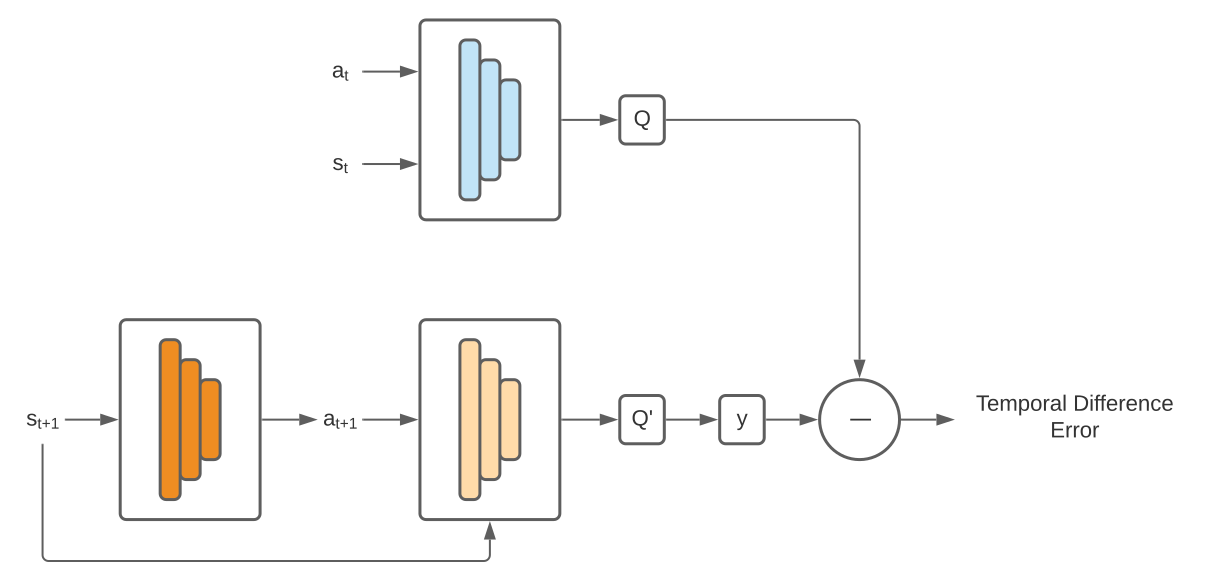
\includegraphics[width=0.7\textwidth]{DDPG.png}
    \caption{Network Architecture of the DDPG Algorithm with Actor and Critic Networks \\ \emph{Note:} TD Error = Temporal Difference Error}
\end{figure}

A common failure mode for DDPG is that the learned Q-function begins to dramatically overestimate Q-values, which then leads to the policy breaking, because it exploits the errors in the Q-function.  Various algorithms have improved stability by addressing well identified issues. One of them is Twin Delayed Deep Deterministic policy gradient (TD3) \cite{fujimoto_addressing_2018}, which uses learns two Q-functions instead of one (hence “twin”), and uses the smaller of the two Q-values to form the targets in the Bellman error loss functions besides other optimizations.

\begin{figure}[h!]
    \centering
    \includegraphics[width=0.7\textwidth]{TD3.png}
    \caption{Network Architecture of the TD3 Algorithm with Twin Actor and Critic Networks \\ \emph{Note:} TD Error = Temporal Difference Error}
\end{figure}

As mentioned before, we find are finding a policy that maximises the expected return, \(R\).

\begin{equation}
    \mathcal{J}(\pi_{\theta}) = \mathbb{E}_{S, A, R \sim \pi_{\theta}} \left[ R \right] \end{equation}

\pagebreak

\section{Training the Model}

\begin{lstlisting}[language=Python]
class SimpleSupplyChain(gym.Env):
    def __init__(self, config):
        self.reset()
        self.action_space = Box(low=0.0, high=10.0)
        self.observation_space = Box(low=-10000, high=10000)

    def reset(self):
        self.supply_chain = SupplyChainEnvironment()
        self.state = self.supply_chain.initial_state()
        return self.state.to_array()

    \item autoscaler
    def step(self, action):
        action_obj = Action(self.supply_chain.warehouse_num)
        action_obj.production_level = action[0]
        action_obj.shippings_to_warehouses = action[1:]
        self.state, reward, done = self.supply_chain.step(
            self.state, action_obj)
        return self.state.to_array(), reward, done, {}
\end{lstlisting}

Finally, we use the Stable Baselines 3 package to create our algorithms and policies. Stable Baselines 3 uses a PyTorch backend to setup its Deep Neural Networks, and the same can be leveraged to create customm policies for our agents. The setup we used is as follows:

\begin{lstlisting}[language=Python]
def train_td3(timesteps: int = 5e5, policy: Union[str | torch.nn] = "MlpPolicy"):
    env = SimpleSupplyChain()

    n_actions = env.action_space.shape[-1]
    action_noise = NormalActionNoise(mean=np.zeros(n_actions), 
                                     sigma=0.1 * np.ones(n_actions))

    agent = TD3(policy=policy, env=env,
                action_noise=action_noise, verbose=1, 
                tensorboard_log="./tensorboard/TD3")

    agent.learn(total_timesteps=timesteps, log_interval=10)
    agent.save()

    return agent
\end{lstlisting}

\subsection{Inference from the Model}
The parameters of the model are saved in a standard PyTorch model file after training is completed and the same can be loaded. This model needs a state array that can be generated with the available data. This state array can be passed to the \lstinline{agent.predict(obs)} method that returns an action that need to be taken in the format specified in the transitions equation.

This same method can be used to generate a graph based visualization of the available stocks in the warehouse, and shipments and hence calculate the profits and cumulative profits.

\begin{lstlisting}[language=Python]
def test_agent(agent, num_episodes=100):
    env = SimpleSupplyChain()

    for episode in range(num_episodes):
        obs = env.reset()
        total_reward = 0
        done = False

        while not done:
            action, _states = agent.predict(obs)
            obs, reward, done, info = env.step(action)

            total_reward += reward
\end{lstlisting}


\pagebreak

\section{Results}
We ran the model with different parameters and hidden layers. A similar random search based on heuristics can be considered for any other usecase. We compared our model to a baseline (s, Q)-policy which gave mean returns of $5488.21$ in our experimentation. Our model with $(300, 400)$ actor hidden layers and $(300, 400)$ critic hidden layers, gave a mean return of $7041.44$, which is an increase of approximately $28.29\%$.

\begin{figure}[h!]
    \centering
    \includegraphics[width=\textwidth]{rewardviolinplot.png}
    \caption{Violin Plot of the rewards obtained from all model architectures over 1000 episodes.}
\end{figure}

\begin{figure}[h!]
    \centering
    \includegraphics[width=\textwidth]{rewardboxplot.png}
    \caption{Box Plot of the rewards obtained from the best model architectures over 1000 episodes.}
\end{figure}



\subsection{Challenges to overcome}

\subsubsection{Switching Platofrms from RLLib to Stable Baselines 3}
RLLib is a great package for Deep Reinforcement Learning, providing a large variety of customizations, algorithms and hyperparameters when selecting a policy. However, configuration of the agent is a mammoth task, and the method of configuration makes it even harder. RLLib is built on top of Ray which is primarily used as an autoscaler when the intention is to deplot the model on the cloud. Owing to the same, Model Training when on a single system is extremely slow and requires constant monioring for errors due to the autoscaler. Moreover, it is based primarily on Tensorflow 1, which makes the codebase even harder to work with. Even though our exploration started with RLLib, maintaining and refactoring the code became a libaility. Further, we could not get inference to work consistently.

Due to these reasons, we made the choice to switch to Stable Baselines 3 by OpenAI. It provides sane defaults and starting points, easy inference and policies written in PyTorch. This helped us with ease of starting out, much faster training of equivalent models (1hour on Stable Baselines 3, vs 8 hours on average on RLLib) and inference worked out of the box. Stable Baselines 3 must be the defacto choice going forward.


\subsubsection{Starting the Tensorboard Dashboard}
Training on Google Colab is the sanest option for most people since they do not have access to GPUs. While on a location machine Tensorboard is the default choice for keeping track of training progress, setting it up on Google Colab is slightly tricky at first, but easy if executed properly.

Load the Tensorboard extension provided by Colab using \lstinline{%load_ext tensorboard}. This loads the \lstinline{tensorboard} magics that can be used to open a local tensorboard instance in the Google Colab window itself.

Use \lstinline{tensorboard --logdir ./tensorboard} to point the directory to where Stable Baselines maintains logs. Start training as you would normally, using the train method provided by the Model itself.

\pagebreak

\bibliographystyle{ieeetr}
\bibliography{references}


\pagebreak

\section*{Glossary}
\begin{enumerate}
    \item Reinforcement Learning: An algorithm that makes decisions based on a given state and the expected reward from taking that action. It tries to maximise the reward
    \item Markov Decision Process: A sequence of events in which the future depends only on the current state, not the history.
    \item Observation space: A Vector Space from where the Observations or current State is sampled. The set of all possible States.
    \item Action space: A vector space from which the Actions are sampled. The Set of all possible Actions.
    \item Policy: Guideline on what is the optimal action to take in a certain state with the goal to maximize the total rewards.
    \item On-Policy: Use the deterministic outcomes or samples from the target policy to train the algorithm.
    \item Off-Policy: Training on a distribution of transitions or episodes produced by a different behavior policy rather than that produced by the target policy.
    \item Action Noise: Minor Disturbances added to the actions in hopes of the model taking actions that it otherwise never would.
    \item Exploration vs Exploitation: The Dilemmma of whether to carry on with the current policy without divergence, or to explore more of the action space.
\end{enumerate}


\end{document}
